%% ===================================================================
%%  Automated Multi-Label Classification of Temporomandibular Joint
%%  Osteoarthritis Signs from CBCT Using Deep Learning
%%  elsarticle -- review format (double-spaced, line numbers)
%% ===================================================================
\documentclass[review,12pt]{elsarticle}

\usepackage{lineno}
\usepackage{amsmath,amssymb}
\usepackage{graphicx}
\usepackage{booktabs}
\usepackage{multirow}
\usepackage{multicol}
\usepackage{array}
\usepackage{rotating}
\usepackage{xcolor}
\usepackage{url}
\usepackage{hyperref}
\usepackage{siunitx}
\usepackage{caption}
\usepackage{subcaption}
\usepackage[margin=2.54cm]{geometry}

\modulolinenumbers[5]

\journal{Journal of Dentistry}

%% ===================================================================
\begin{document}

\begin{frontmatter}

\title{Automated Multi-Label Classification of Temporomandibular Joint
Osteoarthritis Signs from Cone-Beam Computed Tomography Using Deep
Learning}

%% Authors — replace with actual names
\author[muid]{First Author\corref{cor1}}
\ead{first.author@mahidol.ac.th}

\author[muid]{Second Author}
\author[muid]{Third Author}
\author[muid]{Fourth Author (Corresponding Radiologist)}

\cortext[cor1]{Corresponding author.}

\address[muid]{Department of Oral and Maxillofacial Radiology,
Faculty of Dentistry, Mahidol University, Bangkok, Thailand}

% ----------------------------------------------------------------
\begin{abstract}
\textbf{Objectives:}
Temporomandibular joint osteoarthritis (TMJOA) is diagnosed
radiographically by the presence of one or more morphological signs in
cone-beam computed tomography (CBCT) volumes, yet manual interpretation
is time-consuming and subject to inter-observer variability. This study
aimed to develop and evaluate an automated, end-to-end deep-learning
pipeline for multi-label binary classification of five TMJOA signs---
osteoarthritis (OA), condylar erosion, generalised sclerosis, osteophyte,
and subcortical cyst---directly from 3-D CBCT volumes with minimal human intervention, requiring only image-level diagnostic labels.

\textbf{Methods:}
A dataset of 394 joints (209 patients) was labelled by three experienced
oral and maxillofacial radiologists using DC/TMD criteria, with majority
vote used to establish the gold standard. A three-stage preprocessing
pipeline (automatic mandibular segmentation, condyle-centred cropping, and
HU-based intensity normalisation) was applied to all volumes. Twenty deep
learning architectures were evaluated under two training protocols:
Protocol~1 (informativeness-weighted 2-D sagittal slice sampling with
aggregated inference) and Protocol~2 (a learnable 3-D-to-2-D projection
module feeding a frozen 2-D backbone). A two-stage, transfer-learning
strategy initialising each sign-specific task from an OA-trained model was
employed throughout.

\textbf{Results:}
Protocol~1 achieved a mean area under the receiver-operating
characteristic curve (AUC-ROC) of 0.907 across all architectures and
tasks, outperforming Protocol~2 (mean AUC-ROC 0.840). ConvNeXt-Large
(Protocol~1) delivered the best overall performance with a mean AUC-ROC
of 0.924 and a near-perfect AUC-ROC of 0.99 on the OA task.
YOLOv11x-cls was the only architecture for which Protocol~2 surpassed
Protocol~1 (0.926 vs 0.918). Explainability maps (EigenCAM) confirmed
that the best-performing models attended to anatomically relevant condylar
regions.

\textbf{Conclusions:}
The proposed pipeline enables fully automated, clinician-level multi-label
TMJOA classification from CBCT with no manual landmark selection.
ConvNeXt-Large with informativeness-weighted slice sampling represents a
strong baseline for clinical translation.

\textbf{Clinical Significance:}
This system reduces the annotation burden from bounding-box-level
localisation to image-level labels while achieving robust multi-label
classification, facilitating large-scale screening and reproducible
computer-aided diagnosis of TMJOA.
\end{abstract}

\begin{keyword}
temporomandibular joint \sep
osteoarthritis \sep
cone-beam computed tomography \sep
deep learning \sep
multi-label classification \sep
convolutional neural network \sep
transfer learning
\end{keyword}

\end{frontmatter}

\linenumbers

%% ===================================================================
\section{Introduction}
\label{sec:intro}
%% ===================================================================

\section{Introduction}

Temporomandibular joint osteoarthritis (TMJOA) is a progressive
degenerative condition characterised by the breakdown of articular
cartilage and subchondral bone, with prevalence estimates ranging from approximately 2\% to 16\% of the general population
\cite{Xu2025bibliometric}. Accurate diagnosis requires integration of clinical findings with imaging, and CBCT-based assessment is considered the reference standard for detecting osseous changes associated with TMJOA
\cite{ahmad2009research,schiffman2014diagnostic}.

Cone-beam computed tomography (CBCT) provides three-dimensional
visualisation of osseous structures with submillimetre resolution at a
radiation dose and cost considerably lower than conventional computed
tomography, and is therefore the established modality for assessing
TMJOA morphology \cite{larheim2015temporomandibular,honey2007accuracy}.
The Diagnostic Criteria for Temporomandibular Disorders (DC/TMD) imaging
protocol identifies four principal radiographic signs of osteoarthritis:
surface erosion, generalised sclerosis, osteophyte formation, and
subchondral cyst. A diagnosis of osteoarthritis is rendered when at
least one of these findings is present
\cite{schiffman2014diagnostic}. Because multiple signs may coexist
within a single joint, the task is inherently a multi-label
classification problem. We adopt a two-level formulation that mirrors
the clinical workflow: a composite osteoarthritis screen determines
whether a joint is affected, and individual-sign predictions then
characterise which specific findings are present. This yields a
five-class multi-label formulation comprising the composite diagnosis and
the four constituent signs.

Manual interpretation of CBCT volumes for TMJOA is labour-intensive,
requiring systematic review of hundreds of slices across sagittal,
coronal, and axial planes, further underscoring the clinical need for
automated decision-support systems. Deep learning has demonstrated
radiologist-level accuracy in a range of dental and craniofacial imaging
tasks \cite{chen2019deep, choi2021artificial,talaat2023artificial}, and systematic
reviews of CBCT-based TMJOA detection report pooled AUC values of
approximately 0.92 \cite{xu2023artificial},
yet heterogeneity in model architectures, imaging modalities, and
labelling standards has limited direct comparisons across studies.

Within CBCT-based approaches, object detection models, particularly the YOLO family, have emerged as the mainstream paradigm, localising and classifying radiographic signs in a single forward pass from manually selected two-dimensional slices \cite{lee2020automated, talaat2023artificial,Mao2025}. However, these models carry a substantial annotation burden, requiring per-sign bounding boxes on each selected slice. Recent foundation models pre-trained on large, diverse datasets offer a way to reduce this cost. In dental imaging specifically, DentalSegmentator \cite{dot2024dentalsegmentator} — an open-source nnU-Net model trained across seven institutions — provides robust fully automatic segmentation of dento-maxillofacial CBCT structures including the mandible, without task-specific retraining. By using this pre-train segmentation model to isolate the condylar region, a localisation and classification pipeline can be constructed using only image-level labels — a substantially lighter annotation requirement than the bounding-box labels demanded by detection approaches.

A further limitation in existing work is how three-dimensional volumetric data are converted into the two-dimensional inputs that the models expect. CBCT produces a full three-dimensional volume, yet many published models are two-dimensional classifiers or detectors trained on manually selected slices. Because slice selection relies on human judgement, it may introduce operator-dependent variability and selection bias, potentially limiting reproducibility across clinical settings. A recent example is the YOLOv10-based study by Mao et al.\ \cite{Mao2025}, which trained and evaluated on 7,357 annotated oblique-sagittal slices drawn from 1,434 joints. The authors noted that two to ten images were collected per case depending on the extent of radiographic signs — a process in which the annotator must first identify candidate slices and then place bounding boxes on each, adding to annotation cost and potentially amplifying selection variability.

Beyond the preprocessing pipeline, selecting a backbone architecture remains a consequential design choice. Transfer learning from models pretrained on large-scale natural image datasets is the dominant strategy for medical image classification given the scarcity of large annotated medical datasets \cite{kim2022transfer}, yet the substantial domain gap between natural and medical images means that pretraining performance does not straightforwardly predict downstream medical imaging performance, and both the pretraining strategy and the source data characteristics can significantly influence transferability \cite{hosseinzadeh2021systematic}. A related challenge is how best to adapt two-dimensional pretrained models to three-dimensional volumetric input — a question that has been approached through strategies ranging from slice sampling to learned projection modules to fully three-dimensional convolutions, but remains largely unexplored in dental imaging. These considerations motivate two research questions: (1)~which backbone architecture best transfers to TMJOA classification from CBCT, and (2)~which volumetric adaptation strategy most effectively leverages two-dimensional pretrained representations for this task?

To address the gaps identified above, we present an end-to-end pipeline that (i) automatically segments the mandible and crops a condyle-centred volume using three-dimensional skeletonisation, (ii) classifies all five DC/TMD targets simultaneously from a single CBCT volume without manual slice selection, and (iii) recovers spatial interpretability through EigenCAM \cite{muhammad2020eigen} activation maps, complementing the coarse anatomical localisation achieved by the segmentation and cropping stages with finer-grained visualisation of the sub-regions driving each prediction. We systematically benchmark 20 deep learning architectures under two complementary training protocols --- two-dimensional informativeness-weighted slice sampling (Protocol~1) and a learnable three-dimensional-to-two-dimensional projection module (Protocol~2) --- evaluated on 271 training, 80 validation, and 43 test joints. To further investigate the volumetric adaptation question, we compare Protocol~1 and Protocol~2 against an additional strategy using ResNet-50 as a common backbone: a fully three-dimensional convolutional network constructed with the MONAI framework. Together, these experiments provide the most comprehensive architecture and adaptation-strategy comparison to date for TMJOA classification from CBCT.

%% ===================================================================
\section{Materials and Methods}
\label{sec:methods}
%% ===================================================================

\subsection{Ethical Approval and Dataset}
\label{sec:data}

This retrospective study was conducted under institutional review board
approval (MU-MOU CoA 2024/018.1804, Mahidol University Faculty of
Dentistry, Bangkok, Thailand). Written informed consent was waived owing
to the retrospective design.

CBCT volumes were acquired on a 3D Accuitomo XYZ scanner (J.~Morita,
Kyoto, Japan) at 90~kVp, 5~mA, with a voxel size of 0.125~mm and a
field of view of 60~$\times$~60~mm centred on the ipsilateral
temporomandibular joint. A total of 394 joints from 209 patients (age
range 18--80~years; mean 45~years; male:female $\approx$~1:6) were
included. Each joint was treated as an independent observation. Exclusion
criteria were: history of mandibular fracture or orthognathic surgery,
developmental anomalies of the condyle, diagnosis of a systemic
inflammatory joint disease (e.g.\ rheumatoid arthritis), and poor
image quality precluding reliable assessment.

The dataset was partitioned at the patient level into training
(271~joints), validation (80~joints), and test (43~joints) sets to
prevent data leakage between joints from the same patient.

\subsubsection{Reference Standard and Inter-Rater Reliability}

Three oral and maxillofacial radiologists with 20--29~years of clinical
and research experience independently labelled each joint for the five
DC/TMD signs (condylar erosion, generalised sclerosis, osteophyte,
subcortical cyst, and overall OA) using a standardised scoring sheet. The gold-standard label for each sign was determined by majority vote.

Inter-rater reliability was quantified using Cohen's $\kappa$ for all
pairwise rater combinations, Fleiss' multi-rater $\kappa$, and
Krippendorff's $\alpha$ (Table~\ref{tab:irr}). Performance of each
individual rater against the gold standard is reported in
Table~\ref{tab:rater_vs_gold}. Note that OA was not included in the
inter-rater analysis as it is derived deterministically from the
presence of any positive sign.

\subsection{Preprocessing Pipeline}
\label{sec:preproc}

All volumes were processed through a three-stage pipeline
(Figure~\ref{fig:pipeline}).

\subsubsection{Stage 1: Mandibular Segmentation}

Automatic segmentation of the mandible was performed using
DentalSegmentator \cite{dot2024dentalsegmentator}, a publicly available
pre-trained nnU-Net \cite{isensee2021nnu} model fine-tuned on a multi-centre
dental CBCT dataset. No further fine-tuning was performed. The segmentation
mask was used exclusively to define the bounding geometry of the mandible
in subsequent steps; no manual correction was applied to imperfect segmentation outputs, deliberately simulating the conditions of real-world clinical deployment where post-hoc mask editing is impractical.

\subsubsection{Stage 2: Condyle-Centred Cropping}

The condylar centre was identified via 3-D skeletonisation of the
mandibular mask using the \texttt{morphology.skeletonize} function from
scikit-image \cite{van2014scikit}. The skeleton was traversed to identify
the most superior branch tip, taken as a proxy for the condylar process
apex. A $256 \times 256 \times 256$~voxel region of interest was then
extracted, centred on this point.

\subsubsection{Stage 3: Intensity Normalisation}

Hounsfield unit (HU) values were windowed to the range $[-400, 1600]$
to encompass soft-tissue and cortical bone intensities relevant to
condylar morphology, then linearly rescaled to $[0, 1]$. Processed
volumes were saved in NIfTI format.

\subsection{Classification Framework}
\label{sec:framework}

\subsubsection{Task Definition}

For each condylar volume, the model predicted five independent binary
labels corresponding to the DC/TMD signs. The class distributions in the
training set were: OA 238 positive / 156 negative, erosion 218/176,
generalised sclerosis 69/325, osteophyte 182/212, and subcortical cyst
117/277 (Figure~\ref{fig:label_dist}). Note that generalised sclerosis and subcortical cyst are
substantially imbalanced.

\subsubsection{Loss Function and Optimisation}

Binary cross-entropy with logits (\texttt{BCEWithLogitsLoss}) with
class-frequency weighting for generalised sclerosis and subcortical cyst. All models were
optimised with stochastic gradient descent (SGD) with cosine annealing
of the learning rate. Preliminary experiments with unfreezing the
backbone degraded validation performance; consequently, backbone weights
were frozen throughout and only the classifier head was updated.

\subsubsection{Classifier Head}

A shared multi-layer perceptron head (fully connected layers
$512 \to 256 \to n_\text{classes}$ with ReLU activations and dropout
$p = 0.3$) was attached to the pooled feature representation of each
backbone.

\subsubsection{Two-Stage Training Strategy}

To leverage the coarse-to-fine relationship among the labels---OA is
positive whenever any other sign is present---a two-stage transfer
strategy was adopted. In Stage~1, the head was trained for the OA binary
task. In Stage~2, the OA-trained head weights were used to initialise
the heads of the four sign-specific tasks (erosion, sclerosis, osteophyte,
cyst), which were then fine-tuned independently. This curriculum
facilitates learning in the presence of class imbalance by providing an
informed starting point for the minority-class tasks.

\subsection{Protocol 1: Informativeness-Weighted 2-D Slice Sampling}
\label{sec:proto1}

In Protocol~1, each 3-D volume was treated as a pool of 2-D sagittal
slices. An \emph{informativeness score} was defined for each slice as
the ratio of the condylar cross-sectional area (non-zero voxels in the
mandibular mask) to the total slice area:
\begin{equation}
  s_i = \frac{\text{segmented condylar area in slice } i}{\text{image size}}.
  \label{eq:info}
\end{equation}
During training, a single slice was sampled from the volume with
probability proportional to $s_i$, encouraging the model to learn from
slices rich in condylar anatomy. Grayscale slices were replicated to
three channels to match ImageNet-pretrained backbone input requirements.
The largest publicly available variant of each architecture was used
(Table~\ref{tab:models}).

\textbf{Training:} SGD with initial learning rate $10^{-2}$, cosine
annealing, batch size~8, 1000~epochs per task. Because slice sampling
is stochastic, validation was performed three times per epoch and the
scores averaged to obtain a more stable estimate of generalisation.

\textbf{Inference:} All 256 sagittal slices were passed through the
frozen model independently. Slice-level predictions were combined into
a volume-level probability using an informativeness-weighted average:
\begin{equation}
  \hat{p} = \frac{\sum_{i=1}^{256} s_i \cdot \sigma(\hat{y}_i)}
                 {\sum_{i=1}^{256} s_i},
  \label{eq:agg}
\end{equation}
where $\sigma(\cdot)$ is the sigmoid function and $\hat{y}_i$ is the
logit for slice~$i$. The classification threshold was set at the value
maximising Youden's J statistic on the validation set for each task.

\subsection{Protocol 2: Learnable 3-D-to-2-D Projection}
\label{sec:proto2}

Protocol~2 introduced a trainable \texttt{Conv3Dto2DProjection} module
that compressed the 3-D volume into a pseudo-2-D representation suitable
for a standard 2-D backbone. The module consisted of three 3-D
convolutional blocks followed by a learned depth-squeeze operation and
two 2-D convolutional layers, yielding a $3 \times 256 \times 256$
output that mimics a three-channel image. The 2-D backbone was then
applied in a frozen state.

To keep total model size manageable on available hardware (NVIDIA L4 GPU,
Google Colab), architectures were capped at approximately 40 million
parameters; for each architecture family, the variant closest to this
ceiling was selected (Table~\ref{tab:models}).

\textbf{Training:} SGD with initial learning rate $10^{-2}$, cosine
annealing, batch size~4, 200~epochs per task.

\subsection{Model Zoo}
\label{sec:models}

Twenty architectures spanning CNNs, lightweight mobile networks,
vision transformers, and hybrid models were evaluated under both
protocols (Table~\ref{tab:models}). Architectures included ConvNeXt,
DenseNet, EfficientNet, EfficientNet V2, GoogLeNet, Inception V3,
MaxViT, MNASNet, MobileNet V2, MobileNet V3, RegNetX, RegNetY, ResNet,
ResNeXt, ShuffleNet V2, Swin Transformer, Swin Transformer V2, VGG,
Vision Transformer (ViT), and YOLOv11x-cls. All backbone weights were initialised from ImageNet pre-training. Pre-trained weights for all architectures except YOLOv11x-cls were sourced from the TorchVision model library \cite{TorchVision}, while YOLOv11x-cls weights were obtained from Ultralytics \cite{yolo11_ultralytics}. If multiple pre-trained weight sets were available for a single architecture variant (e.g.\ weights from different training recipes or augmentation strategies), the checkpoint reporting the highest ImageNet top-1 accuracy was selected to ensure the strongest possible initialisation. Protocol~1 used the largest available variant of each family; Protocol~2 used variants with $\leq 40\text{M}$ parameters.

\subsection{Explainability}
\label{sec:xai}

EigenCAM \cite{muhammad2020eigen}, a gradient-free class activation mapping
method that decomposes feature maps via principal component analysis,
was applied to all Protocol~1 models at inference. Maps were upsampled
to $256 \times 256$ and overlaid on the corresponding sagittal slice
for visual inspection. Qualitative explainability results are reported
for the best-performing model (ConvNeXt-Large, Protocol~1).

\subsection{Evaluation Metrics}
\label{sec:metrics}

Performance was evaluated on the held-out test set (43~joints) using
accuracy, precision, recall (sensitivity), F1 score and area under the
receiver-operating characteristic curve (AUC-ROC). Task-level means and grand means
(averaged across models) are reported. Because of the class imbalance,
particular emphasis is placed on AUC-ROC as
threshold-independent metrics.

\subsection{Implementation Details}
\label{sec:impl}

All models were implemented in Python using PyTorch~2.9.0+cu128 \cite{paszke2019pytorch}, the Ultralytics library~8.4.14 \cite{yolo11_ultralytics} (for YOLOv11 variants), and MONAI~1.5.2 \cite{monai2026} for volumetric data handling. Visual inspection of raw CBCT volumes and preprocessed outputs at each pipeline stage was performed using 3D Slicer~5 \cite{Slicer2021}, an open-source medical image computing platform. Training was performed on an NVIDIA~L4 GPU (Google Colaboratory); each protocol--task combination required approximately 4--6~hours of wall-clock time.

\subsection{Native 3-D Baseline: MONAI ResNet50}
\label{sec:monai3d}

To contextualise the 2-D and pseudo-2-D approaches in Protocol~1 and
Protocol~2, a native 3-D ResNet50 baseline was trained directly on the
full $256 \times 256 \times 256$ condylar volumes using the MONAI
framework \cite{monai2026}. Unlike Protocol~1 and Protocol~2, this model
processes the entire volumetric input in a single forward pass without
any dimensionality reduction or slice sampling, representing the most
straightforward application of a deep learning classifier to 3-D CBCT
data. The architecture followed the standard ResNet50 design with 3-D
convolutional kernels throughout, initialised with random weights as
no volumetric ImageNet-equivalent pre-training was available. The same
two-stage training strategy, loss function, classifier head, and
SGD optimiser with cosine annealing were applied for consistency;
batch size was set to~2 owing to GPU memory constraints imposed by the
full volumetric input.

%% ===================================================================
\section{Results}
\label{sec:results}
%% ===================================================================

\subsection{Inter-Rater Reliability and Rater Performance}
\label{sec:irr_results}

Inter-rater reliability statistics are presented in
Table~\ref{tab:irr}. Agreement for condylar erosion was excellent
across all metrics (Fleiss' $\kappa = 0.844$; Krippendorff's
$\alpha = 0.844$). Osteophyte showed similarly strong agreement
(Fleiss' $\kappa = 0.837$). Agreement was moderate for generalised
sclerosis (Fleiss' $\kappa = 0.664$) and subcortical cyst (Fleiss'
$\kappa = 0.648$).

Performance of each rater against the gold standard is summarised in
Table~\ref{tab:rater_vs_gold}. All three raters achieved high accuracy
($\geq 0.91$) and recall ($\geq 0.93$) for erosion and osteophyte.
Performance was more variable for generalised sclerosis, where Rater~1
achieved an F1 of 0.667 vs.\ 1.000 for Rater~3, reflecting the
inherent ambiguity of this sign.

\subsection{Overall Protocol Comparison}
\label{sec:proto_compare}

Averaged across all 20 architectures and five tasks, Protocol~1
(2-D slice sampling) achieved a mean AUC-ROC of \textbf{0.907} compared
with \textbf{0.840} for Protocol~2 (3-D projection), a difference of
0.067 AUC units (Figure~\ref{fig:roc}). Protocol~1 also outperformed Protocol~2 on mean
accuracy (0.783 vs.\ 0.728), F1 (0.747 vs.\ 0.687), and PR-AUC
(0.798 vs.\ 0.737). Protocol~2 exceeded Protocol~1 for only a single
architecture, YOLOv11x-cls (AUC-ROC 0.926 vs.\ 0.918), suggesting that
YOLO's feature extraction is particularly amenable to the volumetric
projection approach.

\subsection{Model-Level Results}
\label{sec:model_results}

Full per-model, per-task results are provided in
Tables~\ref{tab:results_p1}~and~\ref{tab:results_p2}; mean AUC-ROC rankings across all architectures
are visualised in Figure~\ref{fig:model_comparison}. Key findings are
summarised below.

\textbf{Best overall model.} ConvNeXt-Large under Protocol~1 achieved
the highest mean AUC-ROC across tasks (0.924), with near-perfect
discrimination for OA (AUC-ROC~0.99, PR-AUC~0.99) and strong
performance on erosion (0.95) and osteophyte (0.92). Performance was
lower, as expected, for the imbalanced classes of generalised sclerosis
(0.94) and subcortical cyst (0.82), though both surpass the macro-average.

\textbf{Catastrophic failure of MNASNet under Protocol~2.}
MNASNet (Protocol~2) collapsed to near-chance performance
(mean AUC-ROC~0.528, mean recall~0.504), suggesting that the
architecture's aggressive channel reduction and depthwise separable
convolutions are incompatible with the volumetric projection module,
likely owing to insufficient representational capacity in the projection
stage.

\textbf{Transformer vs.\ CNN.} Swin Transformer and Vision Transformer
performed competitively under Protocol~1 (mean AUC-ROC 0.920 and 0.920,
respectively), but their advantage over lightweight CNNs such as
MobileNet V2 (0.914) was modest, indicating that ImageNet-pretrained
CNN features transfer effectively to this domain even without
architectural complexity.

\textbf{Generalised sclerosis.} This sign proved most challenging across
all models and both protocols. The macro-average precision for
generalised sclerosis was 0.386 (Protocol~1) and 0.301 (Protocol~2),
attributed to the severe class imbalance (69 positive vs.\ 325 negative
in the training set) and the subtle, diffuse nature of the radiographic
finding.

\subsection{Task-Level Summary}
\label{sec:task_summary}

Across all Protocol~1 models, mean per-task AUC-ROC values were: OA
0.960, erosion 0.931, generalised sclerosis 0.905, osteophyte 0.920, and
subcortical cyst 0.819. The consistently high OA AUC-ROC reflects the
binary, inclusive nature of the label (positive if any sign present),
as well as the frequent co-occurrence of multiple signs within a single
joint (Figure~\ref{fig:venn}). The lower subcortical cyst performance is consistent with its moderate
inter-rater reliability and low prevalence.

\subsection{Explainability}
\label{sec:xai_results}

EigenCAM visualisations for ConvNeXt-Large (Protocol~1) are shown in
Figure~\ref{fig:eigencam}. For joints classified as positive for erosion
and osteophyte, activation was concentrated on the anterosuperior
condylar surface, consistent with the predominant anatomical location
of these findings. For sclerosis, activation was more diffuse, spanning
the subchondral bone plate. Visualisations for joints with false
negatives revealed that uninformative (near-blank) slices occasionally
received high aggregated weight due to imperfect informativeness scoring,
suggesting a direction for future refinement.

\subsection{Native 3-D Baseline Comparison}
\label{sec:3d_baseline}

Table~\ref{tab:resnet_comparison} presents a direct comparison of
ResNet-family models across all three dimensionality paradigms:
ResNet152 under Protocol~1, ResNet50 under Protocol~2, and the native
3-D MONAI ResNet50. The MONAI ResNet50-3D achieved the highest mean
AUC-ROC among the three (0.938), surpassing both ResNet152-Protocol~1
(0.894) and ResNet50-Protocol~2 (0.902). Performance gains were
particularly pronounced for generalised sclerosis (AUC-ROC 0.968 vs.\
0.820 and 0.860, respectively) and subcortical cyst (0.846 vs.\ 0.810
and 0.790), the two most imbalanced and clinically ambiguous signs.
Recall was uniformly high for the 3-D model across all tasks ($\geq
0.917$), suggesting that volumetric processing captures diffuse
morphological changes that are easily missed when only a subset of
sagittal slices is analysed.

These findings confirm that native 3-D models have a performance
ceiling advantage over 2-D approaches on this task when training data
are sufficient. However, the 3-D ResNet50 was trained from random
initialisation, lacking the benefit of large-scale ImageNet
pre-training that underpins Protocol~1 and Protocol~2. The
performance gap may therefore narrow or reverse with domain-specific
3-D pre-training, and the substantially higher memory and compute cost
of volumetric convolutions ($\sim$4$\times$ longer training time per
epoch at batch size~2) represents a practical barrier to large-scale
architecture search of the kind conducted in this study.

%% ===================================================================
\section{Discussion}
\label{sec:discussion}
%% ===================================================================

This study demonstrates that fully automated, multi-label classification
of TMJOA radiographic signs from CBCT is achievable with clinically
useful accuracy using standard deep learning backbones and image-level
annotations. The principal findings are discussed below.

\subsection{End-to-End Automation and Reduced Annotation Burden}

A key novelty of the proposed pipeline is the elimination of any manual
step between raw CBCT acquisition and final classification output. Prior
work has commonly required manual identification of the condylar
region \cite{ecser2023classification,choi2025artificial} or bounding-box annotation for
object detection networks \cite{Ariji2019,Kuwana2021}. By combining
DentalSegmentator \cite{dot2024dentalsegmentator} for automated mandibular
segmentation with a skeletonisation-based condyle localiser, our approach
requires only image-level binary labels---the standard output of a
clinical radiological report---thus substantially reducing the cost and
expertise required for dataset curation.

The native 3-D MONAI ResNet50 baseline (Section~\ref{sec:monai3d})
further illuminates this picture. Trained from random initialisation
directly on full $256 \times 256 \times 256$ volumes, it achieved a
mean AUC-ROC of 0.938 --- exceeding both Protocol~1 (ResNet152: 0.894)
and Protocol~2 (ResNet50: 0.902) on the same backbone family. This
demonstrates that the volumetric context lost during 2-D slice sampling
or depth projection carries genuine diagnostic signal, particularly for
diffuse signs such as generalised sclerosis and subcortical cyst where
the 3-D model showed the largest advantage. The key caveat is that
the 3-D model trained from scratch, foregoing the strong inductive
biases encoded in ImageNet-pretrained weights that Protocol~1 and
Protocol~2 exploit. Future work pairing native 3-D architectures with
volumetric pre-training---for instance via self-supervised learning on
large CBCT corpora---may close this gap while retaining the benefits
of large-scale representation learning.

\subsection{Informativeness-Weighted Slice Sampling as a Radiologist-Mimicking Strategy}

Protocol~1's consistent superiority over Protocol~2 (mean AUC-ROC
advantage 0.067) supports the hypothesis that informativeness-weighted
2-D slice sampling is an effective strategy for extracting
disease-relevant features from 3-D CBCT volumes using 2-D networks.
The weighting scheme (Equation~\ref{eq:info}) mimics the radiologist's
natural tendency to concentrate attention on slices through the condylar
centre, where morphological signs are most evident. The aggregated
inference (Equation~\ref{eq:agg}) then combines evidence across the
entire volume without requiring a single "best" slice to be
pre-selected, a task that is itself non-trivial to automate.

This approach parallels multiple-instance learning frameworks applied
to other volumetric imaging tasks \cite{ilse2018attention,campanella2019clinical}, but
differs in that our aggregation weights are computed from a simple
geometric prior (condylar cross-sectional area) rather than learned
attention, rendering them interpretable and computationally inexpensive.

\subsection{Why Protocol~2 Underperforms}

The learnable 3-D-to-2-D projection in Protocol~2 was motivated by the
desire to process the full volumetric context in a single forward pass
without incurring the memory overhead of fully 3-D networks. However,
the module must simultaneously learn to compress depth information and
adapt the resulting representation to a frozen 2-D backbone---two
non-trivial objectives that may conflict, particularly with the limited
training data available (271~joints). The catastrophic failure of MNASNet
under Protocol~2 exemplifies this fragility: architectures with limited
parameter budgets in the projection head cannot reliably span the
domain gap between learned depth projections and natural images. Future
work might explore unfreezing the backbone jointly with the projection
module using a lower learning rate, or employing knowledge distillation
from Protocol~1 predictions as a supervision signal for Protocol~2.

\subsection{Architecture Insights}

ConvNeXt-Large's top ranking across tasks is consistent with recent
benchmarks showing that modernised pure-CNN architectures match or exceed
vision transformers on medical imaging tasks with limited training
data \cite{liu2022convnet}. The moderate performance of
large transformers (ViT-L/16, Swin-B) relative to their parameter count
likely reflects the well-documented data-hungry nature of these models,
which benefit more substantially from pre-training at scale and may
require larger fine-tuning datasets to realise their theoretical
advantage \cite{dosovitskiy2020image,raghu2021vision}.

The competitive performance of compact architectures---MobileNet V2
(Protocol~1 AUC-ROC 0.914) and MobileNet V3 (0.910)---has practical
implications: these models can run inference in real time on
commodity hardware, supporting deployment in community dental
clinics or low-resource settings.

\subsection{Generalised Sclerosis: The Difficult Sign}

Generalised sclerosis was consistently the most difficult sign to classify,
exhibiting the lowest precision across virtually all models. Three factors
contribute: (i) severe class imbalance (69 positive vs.\ 325 negative
in training); (ii) the relatively modest inter-rater agreement
(Fleiss' $\kappa = 0.664$), indicating inherent label uncertainty; and
(iii) the diffuse, non-focal nature of the finding, which may not produce
a distinctive local activation pattern detectable by 2-D slice-based
models. Strategies such as oversampling, cost-sensitive loss, or
dedicated 3-D sub-volume analysis of the subchondral bone plate may
improve performance on this sign in future work.

\subsection{Two-Stage Training and Class Imbalance}

The two-stage training strategy---first training on OA (a relatively
balanced class) and then fine-tuning on sign-specific tasks using the
OA-trained weights---provided an informed initialisation that appeared to
mitigate the negative effects of imbalance without requiring explicit
class weighting in the loss. This is consistent with curriculum learning
principles \cite{bengio2009curriculum}, where easy tasks precede difficult ones.
Future work should formally ablate this strategy against single-stage
training and class-weighted loss functions.

\subsection{Comparison with Prior Work}

Direct numerical comparison with prior studies is difficult owing to
differences in dataset size, scanner characteristics, class definitions,
and evaluation protocols. Eşer et al.~\cite{ecser2023classification} reported AUC-ROC
values of 0.4970 for or the classification of temporomandibular joint
osteoarthritis using a 2 steps pipe line with fine-tuned segmentation model for condylar cropping and OA classification; our best model
(ConvNeXt-Large, Protocol~1) matches or exceeds these values while
requiring no manual interaction. Prajapati et al.~\cite{choi2025artificial}
achieved accuracy of 0.85 on a two-class (OA vs.\ non-OA) task from
panoramic radiographs, a simpler formulation than the five-class
multi-label problem addressed here. Studies employing YOLO-based
detection \cite{Ariji2019,Kuwana2021} achieve high precision for
specific signs but require bounding-box annotation and address only
one sign at a time.

\subsection{Limitations}

Several limitations should be noted. First, this is a single-centre
study using a single CBCT scanner; generalisability to other institutions
and acquisition protocols remains to be established. Second, the test set
is relatively small (43~joints), and confidence intervals around point
estimates are correspondingly wide. Third, OA was not included in the
inter-rater reliability analysis because it is derived deterministically
from the other labels; this precludes assessment of rater disagreement
at the top-level diagnostic output. Fourth, the informativeness weighting
in Equation~\ref{eq:info} relies on the quality of the automated
segmentation; segmentation failures may degrade cropping and
weighting accuracy. Finally, clinical validation in a prospective
workflow---integrating the system into a dental radiology reporting
environment---has not been performed.

\subsection{Future Directions}

Priorities for future work include: (i) external validation on
multi-centre, multi-scanner data; (ii) formal ablation of the
two-stage training strategy and the informativeness weighting scheme;
(iii) exploration of 3-D architectures (e.g.\ 3-D ResNet, SwinUNETR)
that process the full volume without depth compression; (iv) integration
with a longitudinal monitoring module to detect disease progression;
and (v) prospective clinical validation with radiologist feedback.

%% ===================================================================
\section{Conclusions}
\label{sec:conc}
%% ===================================================================

We have presented a fully automated end-to-end pipeline for multi-label
binary classification of five DC/TMD radiographic signs of
temporomandibular joint osteoarthritis from CBCT volumes. The pipeline
integrates automated mandibular segmentation, skeletonisation-based
condyle localisation, and deep learning classification without any manual
slice selection or bounding-box annotation. Among 20 architectures
evaluated under two training protocols, ConvNeXt-Large with
informativeness-weighted 2-D slice sampling (Protocol~1) achieved the
highest mean AUC-ROC of 0.924, with near-perfect discrimination for the
overall OA label (AUC-ROC~0.99). Protocol~1 consistently outperformed
the learnable 3-D-to-2-D projection approach (Protocol~2; mean AUC-ROC
0.907 vs.\ 0.840), with the sole exception of YOLOv11x-cls. EigenCAM
explainability maps confirmed that the best models attended to
anatomically plausible condylar regions. These findings support the
feasibility of deploying this system as a computer-aided diagnosis
adjunct to conventional CBCT reporting, with the potential to reduce
diagnostic variability and accelerate large-scale TMJOA screening.

%% ===================================================================
\section*{Conflict of Interest}
The authors declare no conflict of interest.

\section*{Funding}
This research did not receive any specific grant from funding agencies
in the public, commercial, or not-for-profit sectors.

\section*{Data Availability}
The dataset used in this study is not publicly available owing to
patient confidentiality requirements. De-identified summary statistics
and model weights may be made available upon reasonable request.

\section*{Acknowledgements}
The authors thank the clinical staff at the Department of Oral and
Maxillofacial Radiology, Mahidol University Faculty of Dentistry, for
facilitating data collection.

%% ===================================================================
%% TABLES
%% ===================================================================

\clearpage

%% --- Table 1: Inter-rater reliability ---
\begin{table}[htbp]
\centering
\caption{Inter-rater reliability statistics for four TMJOA radiographic
signs. Cohen's $\kappa$ is reported for each pairwise rater combination;
Fleiss' $\kappa$ and Krippendorff's $\alpha$ reflect multi-rater
agreement. OA was excluded as it is derived deterministically.}
\label{tab:irr}
\small
\begin{tabular}{lcccccc}
\toprule
\textbf{Sign} &
\textbf{$\kappa$ R1–R2} &
\textbf{$\kappa$ R1–R3} &
\textbf{$\kappa$ R2–R3} &
\textbf{Mean $\kappa$} &
\textbf{Fleiss' $\kappa$} &
\textbf{Krippendorff's $\alpha$} \\
\midrule
Erosion            & 0.810 & 0.852 & 0.871 & 0.844 & 0.844 & 0.844 \\
Generalised Sclerosis & 0.557 & 0.630 & 0.864 & 0.684 & 0.664 & 0.666 \\
Osteophyte         & 0.780 & 0.803 & 0.932 & 0.838 & 0.837 & 0.838 \\
Subcortical Cyst   & 0.670 & 0.629 & 0.645 & 0.648 & 0.648 & 0.649 \\
\bottomrule
\end{tabular}
\end{table}

%% --- Table 2: Rater vs gold standard ---
\begin{table}[htbp]
\centering
\caption{Performance of each individual rater against the majority-vote
gold standard. Acc = accuracy; P = precision; R = recall; F1 = F1 score.}
\label{tab:rater_vs_gold}
\small
\setlength{\tabcolsep}{4pt}
\begin{tabular}{lcccccccccccc}
\toprule
& \multicolumn{4}{c}{\textbf{Rater 1}} &
  \multicolumn{4}{c}{\textbf{Rater 2}} &
  \multicolumn{4}{c}{\textbf{Rater 3}} \\
\cmidrule(lr){2-5}\cmidrule(lr){6-9}\cmidrule(lr){10-13}
\textbf{Sign} & Acc & P & R & F1 & Acc & P & R & F1 & Acc & P & R & F1 \\
\midrule
Erosion
  & 0.947 & 0.900 & 1.000 & 0.947
  & 0.957 & 0.977 & 0.933 & 0.955
  & 0.979 & 1.000 & 0.956 & 0.977 \\
Gen.\ Sclerosis
  & 0.926 & 0.500 & 1.000 & 0.667
  & 0.979 & 0.778 & 1.000 & 0.875
  & 1.000 & 1.000 & 1.000 & 1.000 \\
Osteophyte
  & 0.915 & 0.829 & 0.971 & 0.895
  & 0.979 & 0.971 & 0.971 & 0.971
  & 0.989 & 0.972 & 1.000 & 0.986 \\
Subcortical Cyst
  & 0.946 & 0.889 & 0.842 & 0.865
  & 0.936 & 0.760 & 1.000 & 0.864
  & 0.936 & 0.842 & 0.842 & 0.842 \\
\bottomrule
\end{tabular}
\end{table}

%% --- Table 3: Model zoo ---
\begin{table}[htbp]
\centering
\caption{Architectures evaluated under Protocol~1 (largest variant) and
Protocol~2 ($\leq$40M parameters variant). Param.\ counts are approximate.}
\label{tab:models}
\small
\begin{tabular}{lll}
\toprule
\textbf{Architecture Family} &
\textbf{Protocol~1 Variant} &
\textbf{Protocol~2 Variant} \\
\midrule
ConvNeXt          & convnext\_large      & convnext\_tiny \\
DenseNet          & densenet201          & densenet161 \\
EfficientNet      & efficientnet\_b7     & efficientnet\_b5 \\
EfficientNet V2   & efficientnet\_v2\_l  & efficientnet\_v2\_s \\
GoogLeNet         & googlenet            & googlenet \\
Inception V3      & inception\_v3        & inception\_v3 \\
MaxViT            & maxvit\_t            & maxvit\_t \\
MNASNet           & mnasnet1\_3          & mnasnet1\_3 \\
MobileNet V2      & mobilenet\_v2        & mobilenet\_v2 \\
MobileNet V3      & mobilenet\_v3\_large & mobilenet\_v3\_large \\
RegNetX           & regnet\_x\_32gf      & regnet\_x\_3\_2gf \\
RegNetY           & regnet\_y\_128gf     & regnet\_y\_3\_2gf \\
ResNet            & resnet152            & resnet50 \\
ResNeXt           & resnext101\_64x4d    & resnext50\_32x4d \\
ShuffleNet V2     & shufflenet\_v2\_x2\_0 & shufflenetv2\_x2\_0 \\
Swin Transformer  & swin\_b              & swin\_t \\
Swin Transformer V2 & swin\_v2\_b        & swin\_v2\_t \\
VGG               & vgg19\_bn            & vgg19\_bn \\
Vision Transformer & vit\_l\_16          & vit\_b\_16 \\
YOLOv11           & yolo11x-cls          & yolo11x-cls \\
\bottomrule
\end{tabular}
\end{table}

%% --- Table 4: Full results Protocol 1 ---
\begin{sidewaystable}[htbp]
\centering
\caption{Test-set performance of all 20 architectures under Protocol~1
(informativeness-weighted 2-D slice sampling). Best AUC-ROC per task in
\textbf{bold}. Acc = accuracy; P = precision; R = recall; AUC = AUC-ROC.}
\label{tab:results_p1}
\scriptsize
\setlength{\tabcolsep}{3pt}
\begin{tabular}{l rrrrr rrrrr rrrrr rrrrr rrrrr}
\toprule
& \multicolumn{5}{c}{\textbf{OA}}
& \multicolumn{5}{c}{\textbf{Erosion}}
& \multicolumn{5}{c}{\textbf{Gen.\ Sclerosis}}
& \multicolumn{5}{c}{\textbf{Osteophyte}}
& \multicolumn{5}{c}{\textbf{Subcortical Cyst}} \\
\cmidrule(lr){2-6}\cmidrule(lr){7-11}\cmidrule(lr){12-16}\cmidrule(lr){17-21}\cmidrule(lr){22-26}
\textbf{Model}
& Acc & P & R & F1 & AUC
& Acc & P & R & F1 & AUC
& Acc & P & R & F1 & AUC
& Acc & P & R & F1 & AUC
& Acc & P & R & F1 & AUC \\
\midrule
ConvNeXt       & .95 & .93 & 1.0 & .96 & \textbf{.99} & .91 & .95 & .88 & .91 & .95 & .63 & .30 & 1.0 & .47 & .94 & .86 & .81 & .89 & .85 & .92 & .72 & .53 & .77 & .62 & .82 \\
DenseNet       & .91 & .89 & .96 & .92 & \textbf{.99} & .81 & .75 & 1.0 & .86 & .95 & .84 & .50 & .86 & .63 & .91 & .77 & .67 & .95 & .78 & .92 & .72 & .52 & .92 & .67 & .84 \\
EfficientNet   & .93 & .92 & .96 & .94 & .97 & .88 & .88 & .92 & .90 & .91 & .74 & .38 & .86 & .52 & .88 & .79 & .69 & .95 & .80 & .94 & .63 & .43 & .77 & .56 & .78 \\
EfficientNet V2 & .91 & .86 & 1.0 & .93 & .97 & .81 & .81 & .88 & .84 & .93 & .81 & .47 & 1.0 & .64 & .90 & .77 & .68 & .89 & .77 & .92 & .72 & .52 & .92 & .67 & .83 \\
GoogLeNet      & .91 & .86 & 1.0 & .93 & .98 & .88 & .83 & 1.0 & .91 & .93 & .81 & .47 & 1.0 & .64 & .93 & .72 & .63 & .89 & .74 & .91 & .65 & .46 & .92 & .62 & .82 \\
Inception V3   & .58 & .58 & 1.0 & .74 & .71 & .84 & .81 & .92 & .86 & .94 & .77 & .41 & 1.0 & .58 & .91 & .74 & .65 & .89 & .76 & .93 & .58 & .42 & 1.0 & .59 & .85 \\
MaxViT         & .88 & .92 & .88 & .90 & .97 & .88 & .88 & .92 & .90 & .92 & .77 & .41 & 1.0 & .58 & .88 & .74 & .65 & .89 & .76 & .94 & .70 & .50 & .92 & .65 & .82 \\
MNASNet        & .86 & .83 & .96 & .89 & .95 & .84 & .79 & .96 & .87 & .93 & .67 & .33 & 1.0 & .50 & .89 & .77 & .68 & .89 & .77 & .89 & .60 & .42 & .77 & .54 & .80 \\
MobileNet V2   & .93 & .96 & .92 & .94 & .98 & .86 & .85 & .92 & .88 & .93 & .86 & .55 & .86 & .67 & .93 & .74 & .65 & .89 & .76 & .90 & .70 & .50 & .85 & .63 & .83 \\
MobileNet V3   & .91 & .86 & 1.0 & .93 & .98 & .91 & .92 & .92 & .92 & .95 & .65 & .32 & 1.0 & .48 & .89 & .79 & .69 & .95 & .80 & .92 & .65 & .46 & 1.0 & .63 & .81 \\
RegNetX        & .88 & .86 & .96 & .91 & .98 & .91 & .86 & 1.0 & .92 & .94 & .84 & .50 & .71 & .59 & .92 & .81 & .74 & .89 & .81 & .93 & .65 & .46 & .85 & .59 & .81 \\
RegNetY        & .81 & .81 & .88 & .85 & .95 & .79 & .80 & .83 & .82 & .91 & .74 & .38 & .86 & .52 & .84 & .72 & .63 & .89 & .74 & .89 & .63 & .44 & .92 & .60 & .76 \\
ResNet         & .91 & .86 & 1.0 & .93 & .98 & .91 & .88 & .96 & .92 & .93 & .65 & .28 & .71 & .40 & .82 & .84 & .75 & .95 & .84 & .93 & .74 & .56 & .69 & .62 & .81 \\
ResNeXt        & .91 & .92 & .92 & .92 & .98 & .88 & .91 & .88 & .89 & .94 & .70 & .35 & 1.0 & .52 & .90 & .79 & .71 & .89 & .79 & .92 & .67 & .48 & 1.0 & .65 & .84 \\
ShuffleNet V2  & .81 & .76 & 1.0 & .86 & .96 & .86 & .85 & .92 & .88 & .91 & .74 & .39 & 1.0 & .56 & .92 & .79 & .71 & .89 & .79 & .92 & .60 & .42 & .85 & .56 & .78 \\
Swin Trans.    & .86 & .85 & .92 & .88 & .96 & .88 & .88 & .92 & .90 & .93 & .58 & .28 & 1.0 & .44 & .96 & .79 & .71 & .89 & .79 & .92 & .70 & .50 & .92 & .65 & .83 \\
Swin Trans.\ V2 & .91 & .89 & .96 & .92 & .97 & .88 & .85 & .96 & .90 & .92 & .74 & .39 & 1.0 & .56 & .92 & .86 & .81 & .89 & .85 & .92 & .63 & .43 & .77 & .56 & .84 \\
VGG            & .88 & .92 & .88 & .90 & .97 & .81 & .83 & .83 & .83 & .92 & .56 & .27 & 1.0 & .42 & .94 & .74 & .65 & .89 & .76 & .92 & .67 & .48 & .85 & .61 & .83 \\
ViT            & .88 & .83 & 1.0 & .91 & .98 & .91 & .92 & .92 & .92 & .94 & .74 & .39 & 1.0 & .56 & .89 & .81 & .70 & 1.0 & .83 & .95 & .70 & .50 & .85 & .63 & .84 \\
YOLOv11        & .88 & .86 & .96 & .91 & .98 & .88 & .88 & .92 & .90 & .94 & .70 & .35 & 1.0 & .52 & .92 & .77 & .67 & .95 & .78 & .91 & .70 & .50 & 1.0 & .67 & .84 \\
\midrule
\textbf{Mean}  & .875 & .859 & .958 & .904 & .960 & .867 & .857 & .923 & .887 & .931 & .727 & .386 & .943 & .540 & .905 & .781 & .694 & .911 & .789 & .920 & .668 & .477 & .877 & .616 & .819 \\
\bottomrule
\end{tabular}
\end{sidewaystable}

%% --- Table 5: Full results Protocol 2 ---
\begin{sidewaystable}[htbp]
\centering
\caption{Test-set performance of all 20 architectures under Protocol~2
(learnable 3-D-to-2-D projection). Best AUC-ROC per task in \textbf{bold}.
Acc = accuracy; P = precision; R = recall; AUC = AUC-ROC.}
\label{tab:results_p2}
\scriptsize
\setlength{\tabcolsep}{3pt}
\begin{tabular}{l rrrrr rrrrr rrrrr rrrrr rrrrr}
\toprule
& \multicolumn{5}{c}{\textbf{OA}}
& \multicolumn{5}{c}{\textbf{Erosion}}
& \multicolumn{5}{c}{\textbf{Gen.\ Sclerosis}}
& \multicolumn{5}{c}{\textbf{Osteophyte}}
& \multicolumn{5}{c}{\textbf{Subcortical Cyst}} \\
\cmidrule(lr){2-6}\cmidrule(lr){7-11}\cmidrule(lr){12-16}\cmidrule(lr){17-21}\cmidrule(lr){22-26}
\textbf{Model}
& Acc & P & R & F1 & AUC
& Acc & P & R & F1 & AUC
& Acc & P & R & F1 & AUC
& Acc & P & R & F1 & AUC
& Acc & P & R & F1 & AUC \\
\midrule
ConvNeXt        & .88 & .83 & 1.0 & .91 & .97 & .86 & .80 & 1.0 & .89 & .93 & .77 & .40 & .86 & .55 & .83 & .91 & .86 & .95 & .90 & .95 & .63 & .45 & 1.0 & .62 & .81 \\
DenseNet        & .84 & .82 & .92 & .87 & .92 & .79 & .80 & .83 & .82 & .87 & .58 & .28 & 1.0 & .44 & .92 & .79 & .68 & 1.0 & .81 & .93 & .60 & .43 & .92 & .59 & .85 \\
EfficientNet    & .79 & .74 & 1.0 & .85 & .96 & .84 & .81 & .92 & .86 & .92 & .72 & .37 & 1.0 & .54 & .86 & .81 & .72 & .95 & .82 & .93 & .72 & .53 & .77 & .62 & .79 \\
EfficientNet V2 & .74 & .71 & .96 & .81 & .87 & .79 & .78 & .88 & .82 & .82 & .40 & .21 & 1.0 & .35 & .84 & .70 & .64 & .74 & .68 & .88 & .72 & .53 & .62 & .57 & .76 \\
GoogLeNet       & .91 & .89 & .96 & .92 & .98 & .86 & .82 & .96 & .88 & .95 & .56 & .27 & 1.0 & .42 & .83 & .91 & .83 & 1.0 & .90 & .96 & .65 & .46 & .92 & .62 & .81 \\
Inception V3    & .70 & .73 & .76 & .75 & .77 & .67 & .69 & .75 & .72 & .72 & .77 & .40 & .86 & .55 & .83 & .77 & .71 & .79 & .75 & .86 & .65 & .45 & .69 & .55 & .71 \\
MaxViT          & .84 & .91 & .80 & .85 & .92 & .79 & .86 & .75 & .80 & .88 & .67 & .33 & 1.0 & .50 & .86 & .88 & .82 & .95 & .88 & .91 & .70 & .50 & .85 & .63 & .77 \\
MNASNet         & .42 & .50 & .04 & .07 & .56 & .53 & .60 & .50 & .55 & .65 & .30 & .17 & .86 & .29 & .39 & .60 & .54 & .74 & .62 & .65 & .42 & .23 & .38 & .29 & .39 \\
MobileNet V2    & .84 & .85 & .88 & .86 & .93 & .81 & .83 & .83 & .83 & .87 & .40 & .21 & 1.0 & .35 & .90 & .81 & .70 & 1.0 & .83 & .92 & .81 & .65 & .85 & .73 & .80 \\
MobileNet V3    & .79 & .83 & .80 & .82 & .87 & .77 & .77 & .83 & .80 & .84 & .56 & .23 & .71 & .34 & .65 & .74 & .67 & .84 & .74 & .84 & .63 & .43 & .77 & .56 & .68 \\
RegNetX         & .65 & .78 & .56 & .65 & .69 & .51 & .71 & .21 & .32 & .66 & .70 & .25 & .43 & .32 & .50 & .67 & .58 & 1.0 & .73 & .72 & .51 & .33 & .62 & .43 & .58 \\
RegNetY         & .72 & .78 & .72 & .75 & .81 & .67 & .65 & .92 & .76 & .80 & .65 & .30 & .86 & .44 & .90 & .70 & .62 & .79 & .70 & .78 & .74 & .56 & .69 & .62 & .81 \\
ResNet          & .84 & .78 & 1.0 & .88 & .97 & .81 & .75 & 1.0 & .86 & .94 & .58 & .28 & 1.0 & .44 & .86 & .93 & .86 & 1.0 & .93 & .95 & .72 & .52 & .85 & .65 & .79 \\
ResNeXt         & .81 & .90 & .76 & .83 & .90 & .79 & .86 & .75 & .80 & .88 & .70 & .35 & 1.0 & .52 & .86 & .86 & .84 & .84 & .84 & .91 & .67 & .48 & .77 & .59 & .78 \\
ShuffleNet V2   & .84 & .91 & .80 & .85 & .92 & .79 & .74 & .96 & .84 & .90 & .56 & .27 & 1.0 & .42 & .80 & .79 & .73 & .84 & .78 & .88 & .67 & .48 & .85 & .61 & .74 \\
Swin Trans.     & .81 & .81 & .88 & .85 & .94 & .81 & .81 & .88 & .84 & .90 & .53 & .26 & 1.0 & .41 & .93 & .84 & .77 & .89 & .83 & .91 & .74 & .56 & .69 & .62 & .82 \\
Swin Trans.\ V2 & .86 & .95 & .80 & .87 & .97 & .86 & .91 & .83 & .87 & .92 & .77 & .41 & 1.0 & .58 & .91 & .88 & .82 & .95 & .88 & .93 & .63 & .44 & .92 & .60 & .82 \\
VGG             & .77 & .78 & .84 & .81 & .89 & .77 & .77 & .83 & .80 & .84 & .65 & .32 & 1.0 & .48 & .85 & .81 & .76 & .84 & .80 & .94 & .74 & .55 & .92 & .69 & .78 \\
ViT             & .86 & .95 & .80 & .87 & .93 & .84 & .90 & .79 & .84 & .91 & .77 & .41 & 1.0 & .58 & .83 & .86 & .81 & .89 & .85 & .93 & .67 & .48 & .77 & .59 & .82 \\
YOLOv11         & .86 & .83 & .96 & .89 & .97 & .84 & .79 & .96 & .87 & .93 & .60 & .29 & 1.0 & .45 & .88 & .79 & .69 & .95 & .80 & .95 & .74 & .54 & 1.0 & .70 & .90 \\
\midrule
\textbf{Mean}   & .789 & .814 & .812 & .798 & .887 & .770 & .783 & .819 & .789 & .857 & .612 & .301 & .929 & .449 & .812 & .803 & .733 & .898 & .804 & .887 & .668 & .480 & .793 & .594 & .761 \\
\bottomrule
\end{tabular}
\end{sidewaystable}

\begin{table}[htbp]
\centering
\caption{Direct comparison of ResNet-family models across three
dimensionality paradigms on the held-out test set. Acc = accuracy;
P = precision; R = recall; AUC = AUC-ROC. Mean is averaged across
five tasks.}
\label{tab:resnet_comparison}
\small
\setlength{\tabcolsep}{4pt}
\begin{tabular}{llccccc}
\toprule
\textbf{Model} & \textbf{Paradigm} &
\textbf{OA} & \textbf{Erosion} & \textbf{Gen.\ Scl.} &
\textbf{Osteo.} & \textbf{Sub.\ Cyst} \\
& & AUC & AUC & AUC & AUC & AUC \\
\midrule
ResNet152   & Protocol~1 (2-D)       & .98 & .93 & .82 & .93 & .81 \\
ResNet50    & Protocol~2 (pseudo-3D) & .97 & .94 & .86 & .95 & .79 \\
ResNet50-3D & MONAI native 3-D       & .96 & .95 & .97 & .97 & .85 \\
\midrule
\multicolumn{2}{l}{\textbf{Mean AUC-ROC}} & & & & & \\
ResNet152   & Protocol~1 & \multicolumn{5}{c}{0.894} \\
ResNet50    & Protocol~2 & \multicolumn{5}{c}{0.902} \\
ResNet50-3D & MONAI 3-D  & \multicolumn{5}{c}{\textbf{0.938}} \\
\bottomrule
\end{tabular}
\end{table}

%% ===================================================================
%% FIGURES
%% ===================================================================

% \clearpage

\begin{figure}[htbp]
  \centering
  \includegraphics[width=\textwidth]{figures/pipeline.pdf}
  \caption{Overview of the proposed end-to-end pipeline. (A)~Raw CBCT
  volume. (B)~Mandibular segmentation via DentalSegmentator. (C)~Condyle
  localisation via 3-D skeletonisation and $256\times256\times256$
  cropping. (D)~HU windowing and normalisation. (E)~Protocol~1:
  informativeness-weighted sagittal slice sampling and aggregated
  inference. (F)~Protocol~2: learnable 3-D-to-2-D projection feeding a
  frozen 2-D backbone. (G)~Multi-label binary predictions for five
  DC/TMD signs.}
  \label{fig:pipeline}
\end{figure}

\begin{figure}[htbp]
  \centering
  \includegraphics[width=\textwidth]{figures/eigencam.pdf}
  \caption{EigenCAM activation maps for ConvNeXt-Large (Protocol~1) on
  representative test-set joints. Each row shows the most informative
  sagittal slice, the raw EigenCAM heatmap, and the overlay. Columns
  correspond to true-positive classifications for (a)~OA, (b)~condylar
  erosion, (c)~generalised sclerosis, (d)~osteophyte, and
  (e)~subcortical cyst. Activation is concentrated on the condylar
  surface for erosion and osteophyte, and is more diffuse for sclerosis.}
  \label{fig:eigencam}
\end{figure}

\begin{figure}[htbp]
  \centering
  \includegraphics[width=0.9\textwidth]{figures/roc_curves.pdf}
  \caption{Receiver-operating characteristic curves for ConvNeXt-Large
  (Protocol~1, solid) and YOLOv11x-cls (Protocol~2, dashed) across five
  tasks. AUC-ROC values are annotated for each task.}
  \label{fig:roc}
\end{figure}

\begin{figure}[htbp]
  \centering
  \includegraphics[width=0.85\textwidth]{figures/model_comparison.pdf}
  \caption{Mean AUC-ROC (averaged across five tasks) for all 20
  architectures under Protocol~1 (orange) and Protocol~2 (blue). Models
  are sorted by Protocol~1 AUC-ROC in descending order. Error bars
  represent the range across tasks.}
  \label{fig:model_comparison}
\end{figure}

\begin{figure}[htbp]
  \centering
  \includegraphics[width=0.82\textwidth]{figures/label_distribution.pdf}
  \caption{Class distribution across the training, validation, and test
  sets for each of the five classification tasks. Positive (dark) and
  negative (light) counts are shown per split. Note the pronounced
  imbalance for generalised sclerosis (69 positive vs.\ 325 negative
  in training) and subcortical cyst (117 vs.\ 277).}
  \label{fig:label_dist}
\end{figure}

\begin{figure}[htbp]
  \centering
  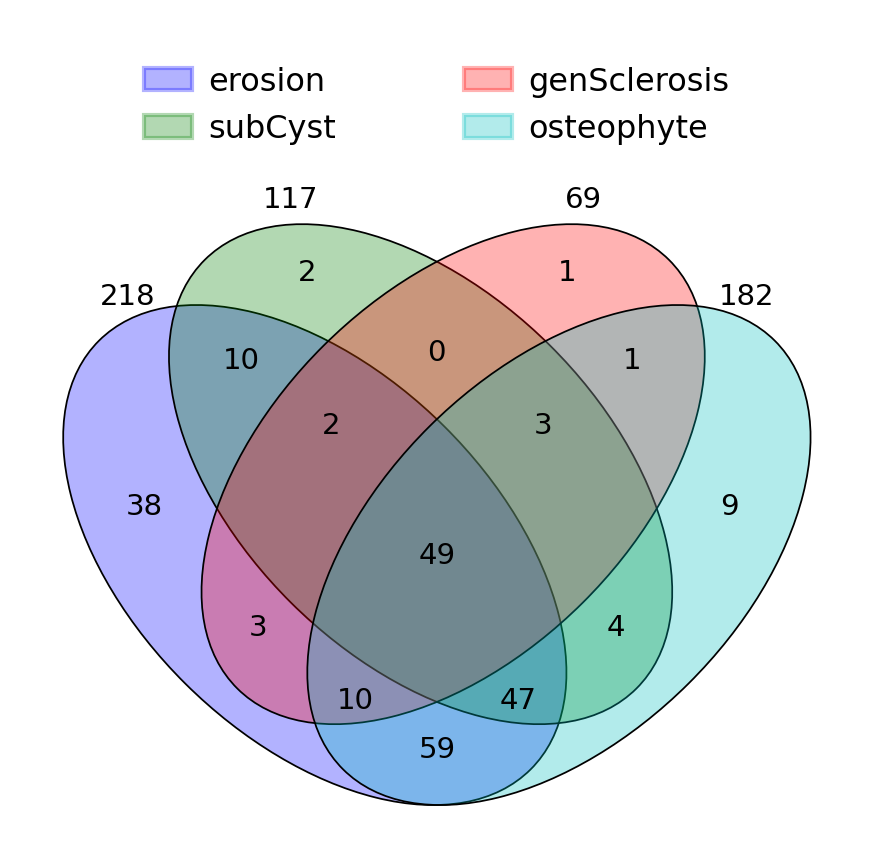
\includegraphics[width=0.72\textwidth]{figures/Venn_4.png}
  \caption{Four-set Venn diagram illustrating the co-occurrence of
  condylar erosion, generalised sclerosis, osteophyte, and subcortical
  cyst among the OA-positive joints in the full dataset. Each region
  displays the number of joints exhibiting that exact combination of
  signs.}
  \label{fig:venn}
\end{figure}

%% ===================================================================
%% REFERENCES
%% ===================================================================
\newpage
\newpage
\bibliographystyle{elsarticle-num}
\bibliography{references}

\end{document}